\documentclass[a4paper,11pt]{article}
\pdfoutput=1 % if your are submitting a pdflatex (i.e. if you have
             % images in pdf, png or jpg format)

\usepackage{jinstpub} % for details on the use of the package, please
                     % see the JINST-author-manual
%\usepackage{amsmath}
\usepackage{heppennames2}
\usepackage{hepnicenames}

%\usepackage{txfonts}
%\usepackage{newtxtext,newtxmath}
\usepackage{mathptmx}

%\usepackage[caption=false]{subfig}
%\usepackage{subfigure}
\usepackage{subcaption}
%\usepackage{feynmp-auto}
\usepackage{color}
\usepackage{gensymb}
\unitlength = 1mm

%\makeatletter
%\def\endfmffile{%
%  \fmfcmd{\p@rcent\space the end.^^J%
%          end.^^J%
%          endinput;}%
%  \if@fmfio
%    \immediate\closeout\@outfmf
%  \fi
%  \ifnum\pdfshellescape=\@ne
%    \immediate\write18{mpost \thefmffile}%
%  \fi}
%\makeatother

\newcommand{\pt}{\ensuremath{p_{\mathrm T}}}

\newcommand{\mh}{\ensuremath{m_{H}} } 
\newcommand{\ptmiss}{\ensuremath{p_{\mathrm T}^{\mathrm{miss}}}}
\newcommand{\chisquare}{\ensuremath{\chi^2}}

\newcommand{\decayElectron}{\Pem\PAGne\PGnGt}
\newcommand{\decayMuon}{\PGmm\PAGnGm\PGnGt}
\newcommand{\decayPion}{\PGpm\PGnGt}
\newcommand{\decayRho}{\PGrP{\PGpm\PGpz}\PGnGt}
\newcommand{\decayAiPhoton}{\PaDoP{\PGpm\PGpz\PGpz}\PGnGt}
\newcommand{\decayAiPion}{\PaDoP{\PGpm\PGpm\PGpp}\PGnGt}
\newcommand{\decayThreePionPhoton}{\PGpm\PGpm\PGpp\PGpz\PGnGt}

\newcommand{\decayElectronShort}{\Pem\PAGne}
\newcommand{\decayMuonShort}{\PGmm\PAGnGm}
\newcommand{\decayPionShort}{\PGpm}
\newcommand{\decayRhoShort}{\PGrP{\PGpm\PGpz}}
\newcommand{\decayAiPhotonShort}{\PaDoP{\PGpm\PGpz\PGpz}}
\newcommand{\decayAiPionShort}{\PaDoP{\PGpm\PGpm\PGpp}}
\newcommand{\decayThreePionPhotonShort}{\PGpm\PGpm\PGpp\PGpz}

\newcommand{\higgsToTauTau}{\PHiggs $\to$ \PGtm \PGtp}
\newcommand{\eeToTauTau}{\Pem\Pep $\to$ \PGtm\PGtp}
\newcommand{\rootS}{\ensuremath{\sqrt{s}} }


\title{\boldmath Reconstruction and classification of tau lepton decays at a future \Pem \Pep Linear Collider}


%% %simple case: 2 authors, same institution
%% \author{A. Uthor}
%% \author{and A. Nother Author}
%% \affiliation{Institution,\\Address, Country}

% more complex case: 4 authors, 3 institutions, 2 footnotes
\author[a,1]{B. Xu,\note{Corresponding author.}}
%\author[a,b,1]{F. Irst,\note{Corresponding author.}}
\author[a]{S. Green,}
\author[a]{J. S. Marshall,}
\author[a]{M. A. Thomson}
%\author[a,2]{T. Hird\note{Also at Some University.}}
%\author[c,2]{and Fourth}

% The "\note" macro will give a warning: "Ignoring empty anchor..."
% you can safely ignore it.

\affiliation[a]{Cavendish Laboratory,\\JJ Thomson Avenue, Cambridge, CB3 0HE, UK}
%\affiliation[b]{Another University,\\different-address, Country}
%\affiliation[c]{A School for Advanced Studies,\\some-location, Country}

% e-mail addresses: only for the forresponding author
\emailAdd{xu@hep.phy.cam.ac.uk}


\abstract
{
Seven tau lepton decay modees were studied using simulated data, for the proposed Compact Linear Collider. 
Tau leptonic physics is important. Its branching ratios measurements provide precision tests of the Standard Model. Spin state of a tau lepton can  be used to measure the CP properties of the Higgs boson, via the Higgs to a tau pair decay.
Correct classification prbability of tau lepton decay is a benchmark of detector performance.
In this paper, seven decay modes were reconstructed and classified for centre of mass of 100, 200, 500 and 1000\,GeV, and for electromagnetic calorimeter (ECal) square cell sizes of 3, 5, 7, 10, 15, and 20\,mm.
Major challenges for classification include reconstucting multiple nearby photons as separate entities, and correct assoication of inner detector tracks to energy deposited in calorimeters. 
Efficient classification of tau decay mode is achieved. Overall tau lepton hadronic decay correct classification probaility is over 90\% for \rootS = 100\,GeV. For \rootS = 200\,GeV, the probability decreases from over 90\% to 86\% for ECal square cell sizes from 3 to 20\,mm. For \rootS = 500 and 1000\,GeV, the probability degrades significantly, from over 90\% to 77\%,  and from 86\% to 75\%, respectively, for the same range of the cell sizes. 
}
\keywords{TODO: Only keywords from JINST's keywords list please}


\arxivnumber{1234.56789} % only if you have one


% \collaboration{\includegraphics[height=17mm]{example-image}\\[6pt]
%   XXX collaboration}
% or
%\collaboration[c]{on behalf of XXX collaboration}


% if you write for a special issue this may be useful
\proceeding{N$^{\text{th}}$ Workshop on X\\
  when\\
  where}



\begin{document}
\maketitle
\flushbottom


\section{Introduction}

The tau lepton has been examined extensively in the past. In particular, detailed studies were performed at the Large Electron Positron Collider (LEP)\cite{Schael:2005am}. The properties of tau lepton decay  provide precision tests of the Standard Model and models beyond the Standard Model. Such properties include tau decay branching ratios, and total tau hadronic decay width, which depends on the strong coupling constant. The spin state of tau lepton, which can be inferred from kinematic properties of tau decay products, can be used to measure the CP (the product of charge conjugation and parity symmetries) of the Higgs, via \higgsToTauTau channel. 

Performance of tau decay mode classcification provides a benchmark of detector performance. Since the tau lepton has a very short lifetime \cite{Abreu:1991jn}, it decays in the inner detector before reaching the calorimeter. Typical tau decay products are charged particles, and multiple photons from \PGpz. Reconstruction of multiple nearby photons requires an excellent electromagnetic calorimeter (ECal) spatial resolution. Separating different charged particle relies on performance of the inner detector tracking system. 

% A previous study was performed with the International Large Detector (ILD) \cite{Abe:2010aa} in the context of the International Linear Collider (ILC) \cite{Brau:2007zza}
The study was done in the context of the CLIC\_ILD detector concept \cite{Linssen:2012hp} with the PandoraPFA software package \cite{Marshall:2015rfa}. The CLIC\_ILD detector concept is designed for the Compact LInear Collider (CLIC) \cite{Linssen:2012hp} based on the ILD detector \cite{Abe:2010aa}. A cross section of the CLIC\_ILD detector is shown in figure~\ref{fig:ILD}. The detector consists of vertex detectors, tracking detectors, electromagnetic calorimeters, hadronic calorimeters (HCal) and muon chambers. Magnetic field is optimised for the particle flow approach (PFA) to calorimetry \cite{Thomson:2009rp} with high granularity in both longitudinal and transverse direction, providing unprecedented jet energy resolutions.

\begin{figure}[htbp]
\centering % \begin{center}/\end{center} takes some additional vertical space

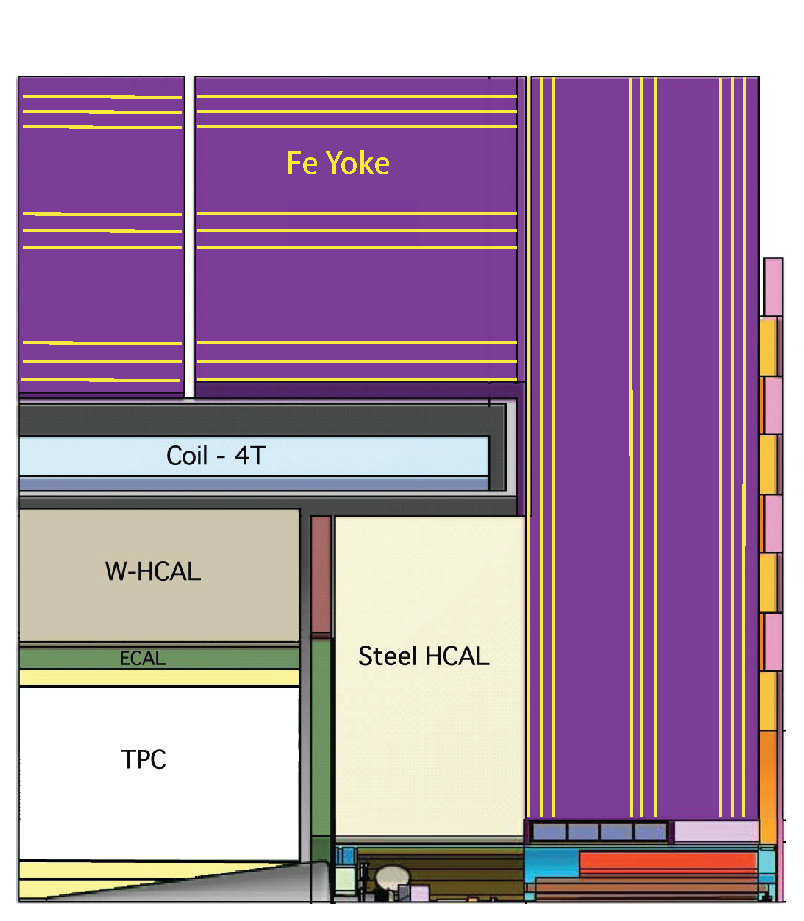
\includegraphics[width=.45\textwidth]{plots/CLICILD.eps}
\qquad
\caption{\label{fig:ILD} Longitudinal cross section of top quadrant of the CLIC\_ILD detector concept, taken from \cite{Linssen:2012hp}
}
\end{figure}

Particle flow approach to calorimetry aims to reconstruct individual particles. This makes an efficient tau decay mode classfication possible. PandoraPFA, \cite{Marshall:2015rfa}, a leading pattern recognition software, has demonstrated it ability to exploit information from high granular calorimeters in the context of future linear colliders. Charged particles are reconstructed by projecting tracks from inner tracking detector and associating calorimeter hits to these tracks. Photons are reconstructed from calroimeter hits in the ECal, with comparision to expected electromagnetic shower profiles. Neutral hadrons are reconstructed from calroimeter hits in the HCal. The output of the PandoraPFA is Particle Flow Object (PFO), which contains energy, momentum, position, particle id and other information.

Ability to separate tau decay modes relies on photon reconstruction. Calorimeter hits in the ECal are clustered and carefully isolated from nearby charged particles. These clusters are compared with expected electromagnetic shower profiles, using a likelihood based classcifier. Separate algorithms split merged photons and combine small photon fragments to main photons. Photon reconstruction in PandoraPFA is described in \cite{Xu:2016rcz}.

%The difficulty of the \PGt decay mode separation is to correctly reconstruct photons in the final states. Two main features of the reconstruction software, PandoraPFA \cite{Marshall:2015rfa}, help to separate the final states. Firstly, the iterative track cluster association algorithms connecting reconstructed tracks to the cluster showers in the calorimeters, providing a good identification of the charged particles and leave a cleaner environment for the neutral particles. Secondly, a transverse calorimeter shower profile based photon reconstruction algorithm carefully identifies and separates nearby photons, using a likelihood photon identification algorithm. Along side with other reconstruction algorithms in the PandoraPFA software, charged particles and photons are well reconstructed and used as inputs for \PGt decay mode separation.

This paper describes the reconstruction and classcification of tau lepton decay modes. The classcification is used for the ECal optimisation, with varying ECal square cell sizes, using different centre of mass energies (\rootS) for \eeToTauTau interaction.


\section{Simulation and Reconstruction}
\label{section:MC}
Simulated Monte Carlo (MC) samples were generated with the generator software WHIZARD 1.95 \cite{whizard}, with PYTHIA 6.4 \cite{Sjostrand:1995iq}  used for the hadronisation and  tuned to the LEP results \cite{}. TAUOLA \cite{Jadach:1993hs} is used to describe the \PGt lepton decays with correct spin correlation between decay products. The initial state radiation (ISR) and the beam induced background were not simulated, but final state radiation (FSR) was simulated. This study is aimed for detector optimisation. Hence a clean detector enviornment is preferred to maximise the effect of the calorimeter design on the performance of the tau decay classcification.

Around two millions \eeToTauTau MC simulated events were gneerated, for each ECal square cell size of 3, 5, 7, 10, 15 and 20 mm, and for each \rootS energy of 100, 200, 500 and 1000\,GeV. In total, 48 millions simulated events were generated. Generated events were considered in the subsequent analysis if they pass a series of generator level selection cuts designed to isolate the effect of the calorimeter design on the performance of the tau decay classcification. Around 60\% of generated events passed the selection cuts.

Events are discarded if simulated photons convert before reaching the calorimeters. Converted photons would not be reconstructed as photons, and events with converted photons would decrease the classification efficiency. That degredation would not be due to the calorimeter design.

Events are also discarded if total energy of the tau lepton visible decay products is less than 5\,GeV. This ensures the decay products properly reconstructed.

Events are further discarded if tau leptons are not with the barrel and end cap calorimeter regions. The polar angle for the end cap region is defined $ 17.2\degree < |\theta_{Z}| < 34.4\degree$. The polar angle for the barrel region is defined $ 45.8\degree < |\theta_{Z}| < 90\degree$. Very forward region of the detector is not simulated dut to technical reasons. The particle reconstruction was not optimised for the gap region between the barrel and the end cap region for the CLIC\_ILD detector. Therefore by confining to the barrel and the end cap region only, a consistent high particle reconstruction efficiency is ensured.


Events were simulated with software MOKKA \cite{MoradeFreitas:2002kj} with the CLIC\_ILD detector geometry description, based on the GEANT 4 package  \cite{Agostinelli:2002hh}. Reconstruction was done with ilcsoft version v01-17-07 \cite{Gaede:82475} and PandoraPFA version v02-02-00 \cite{Marshall:2015rfa}, where the photon reconstruction is described in \cite{Xu:2016rcz}.


\section{Analysis strategy}

\begin{table}[htbp]
\centering
\caption{\label{tab:decay_mode} Branching fractions of the seven \PGtm decays in this study\cite{Agashe:2014kda}. \PGtp decays similarly to \PGtm.}
\smallskip
\begin{tabular}{|l |c|}
\hline
  \textbf{Decay mode} & \textbf{Branching fraction / \%} \\
\hline
  \decayElectron        & 17.83$\pm$0.04   \\
  \decayMuon  	& 17.41$\pm$0.04  \\
  \decayPion     	& 10.83$\pm$0.06   \\
  \decayRho	& 25.52$\pm$0.09 \\
  \decayAiPhoton	& 9.30$\pm$0.11    \\
  \decayAiPion  	    & 8.99$\pm$0.06  \\
  \decayThreePionPhoton  	    & 2.70$\pm$0.08  \\

\hline
\end{tabular}
\end{table}

The  seven tau lepton decay modes were condidered, shown in table~\ref{tab:decay_mode}. These decay modes cover 92.58\,\% of all tau decays. The neglected decay modes each have branching fractions below 1\%. 

%The chosen final states can be classified into three categories: leptonic decays, one-prong with photons and three-prong with photons. 

This study focuses on the reconstuction and classcification of single tau decay. Therefore, two tau leptons in \eeToTauTau channel are separated using thrust variable. Thrust axis is the best fitted line of all particles' momentum. The sign of the dot product between the thrust axis and the particle' momentum separates particles into one of the two collections. Two collections correspond to decay products of two tau leptons. This method is valid because two taus from \eeToTauTau are largely travelling in opposite direction. Formally the definition of  thrust axis is
\begin{equation}
T = max_{\hat{n}} \frac {\sum_i \left| p_i . \hat{n} \right|}{\sum_i \left| p_i \right|} \,,
\end{equation}
where $p_i$ is the particle $i$'s momentum. $\hat{n}$ is the thrust axis.



\begin{figure}[!tbp]
\centering % \begin{center}/\end{center} takes some additional vertical space

%\subfigure[Figure A]{\label{fig:a}\includegraphics[width=60mm]{example-image-a}}

\begin{subfigure}[b]{0.45\textwidth}
 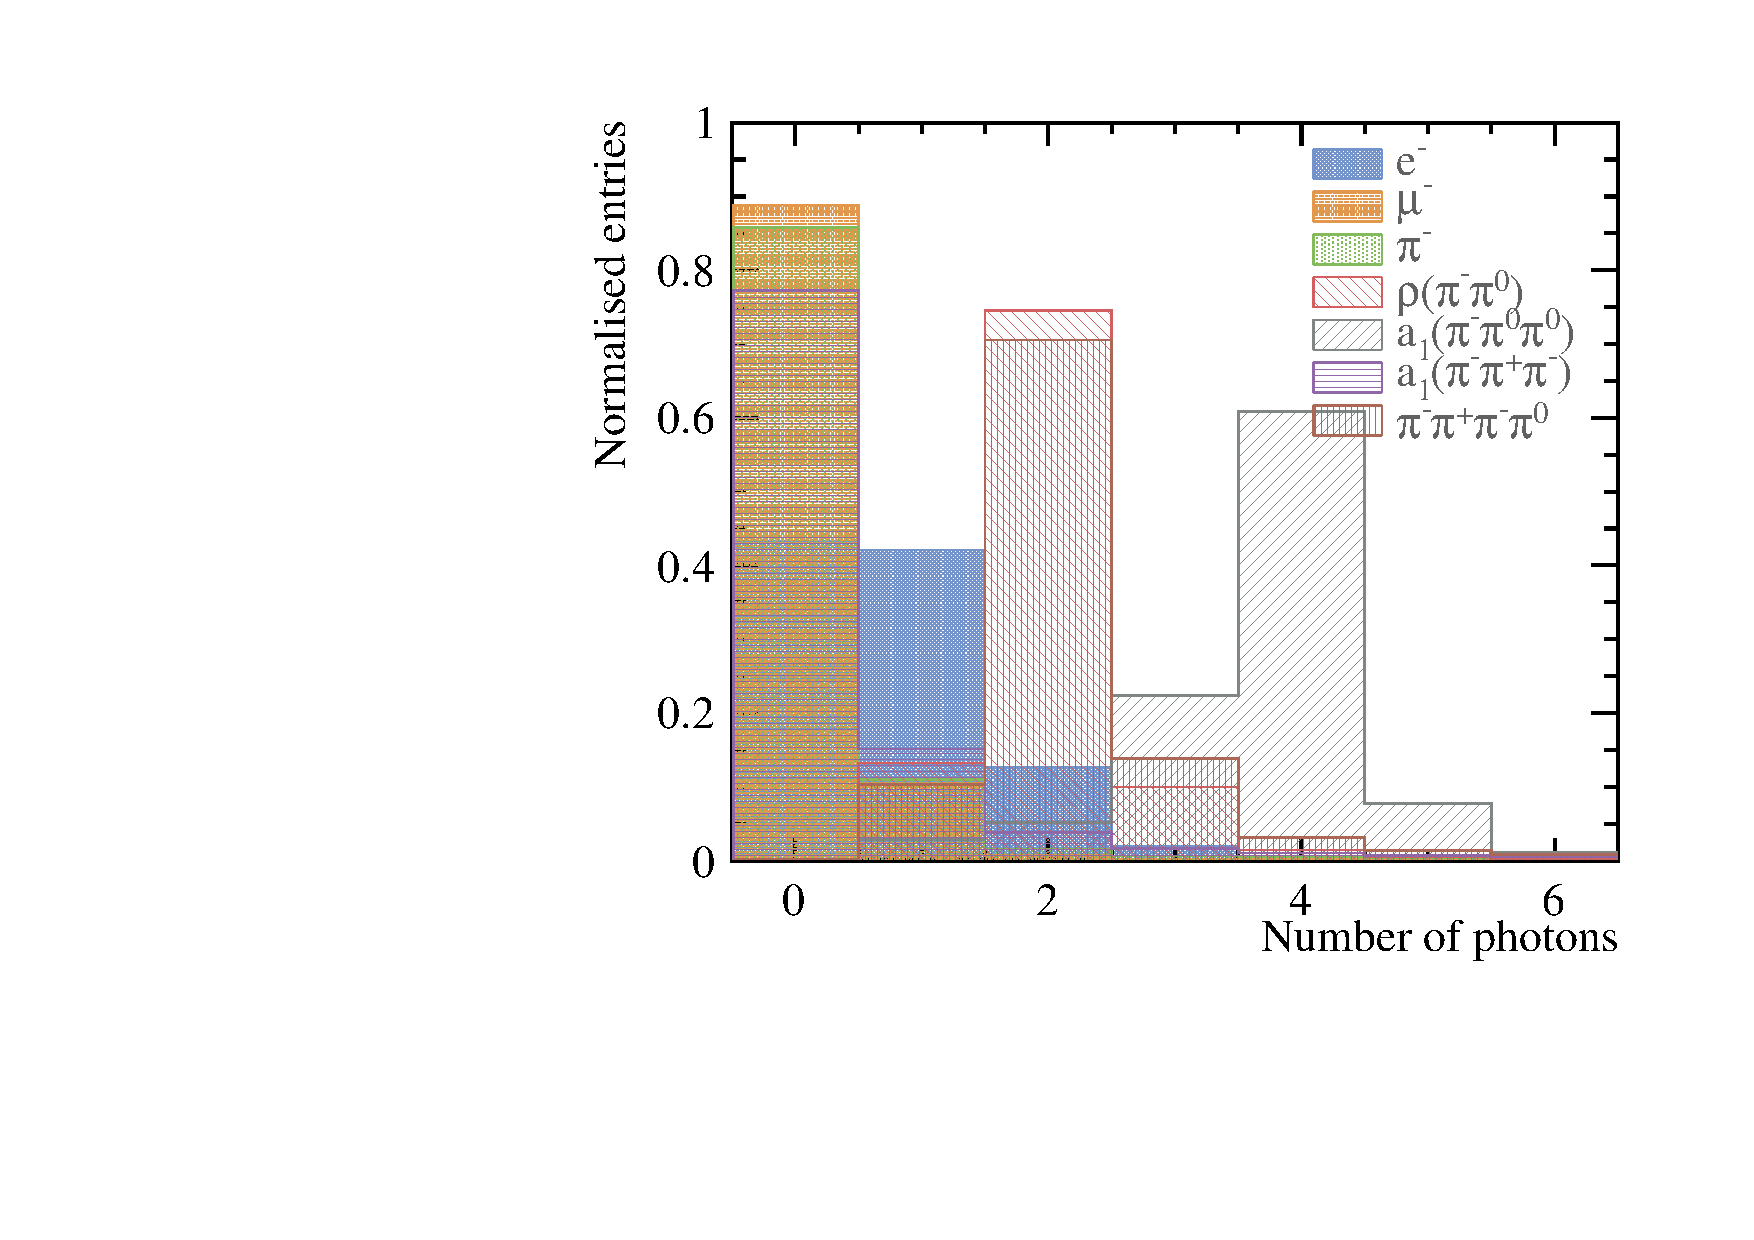
\includegraphics[width=\textwidth]{plots/var/nPhoton_100GeV_improved} 
  \caption{}
  \label{fig:nPfos}
\end{subfigure}
\hfill
\begin{subfigure}[b]{0.45\textwidth}
 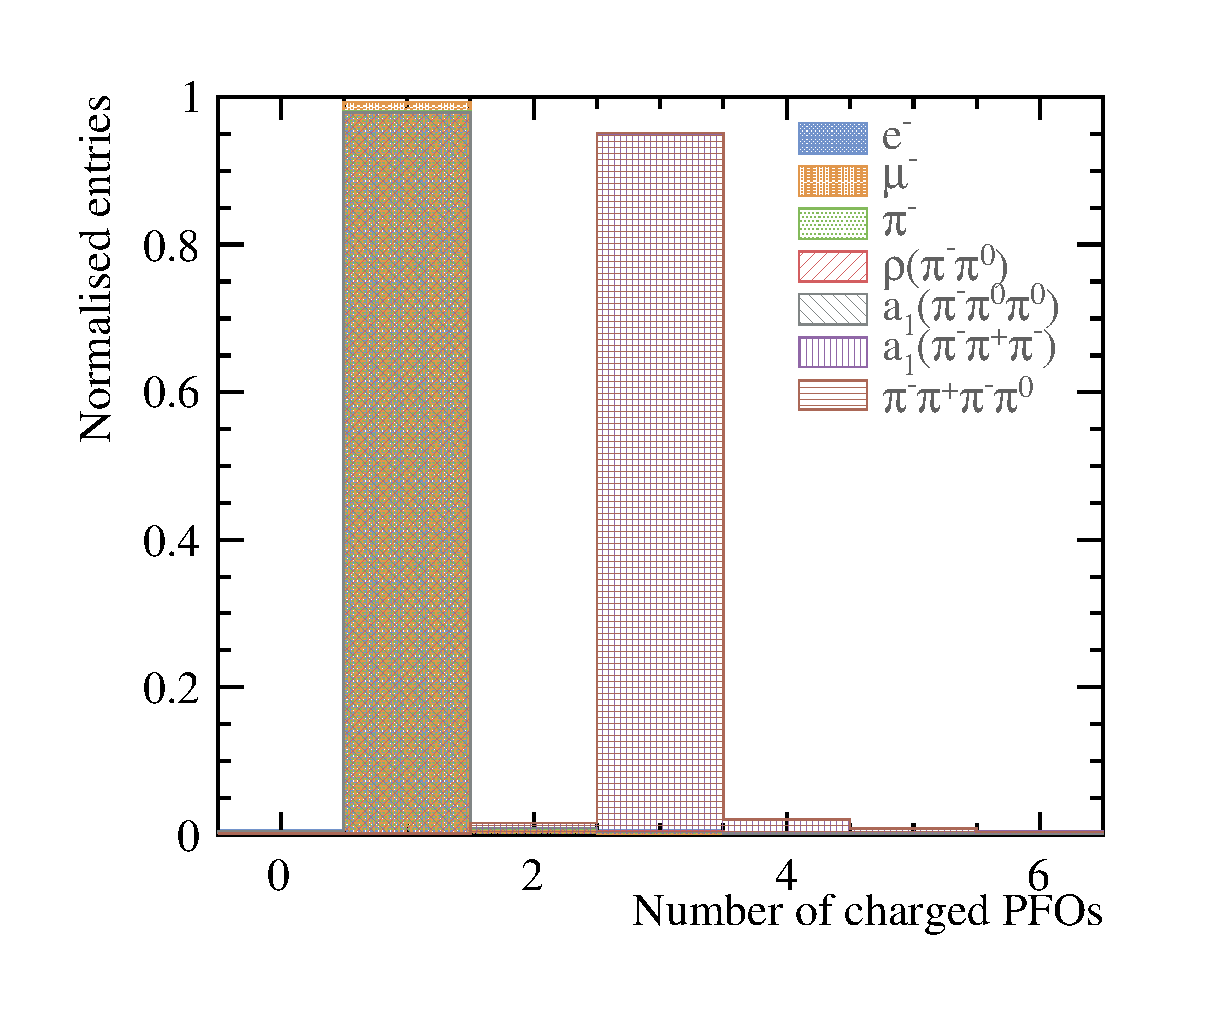
\includegraphics[width=\textwidth]{plots/var/nCharge_100GeV_improved} 
  \caption{}
  \label{fig:nCharge}
\end{subfigure}
\begin{subfigure}[b]{0.45\textwidth}
 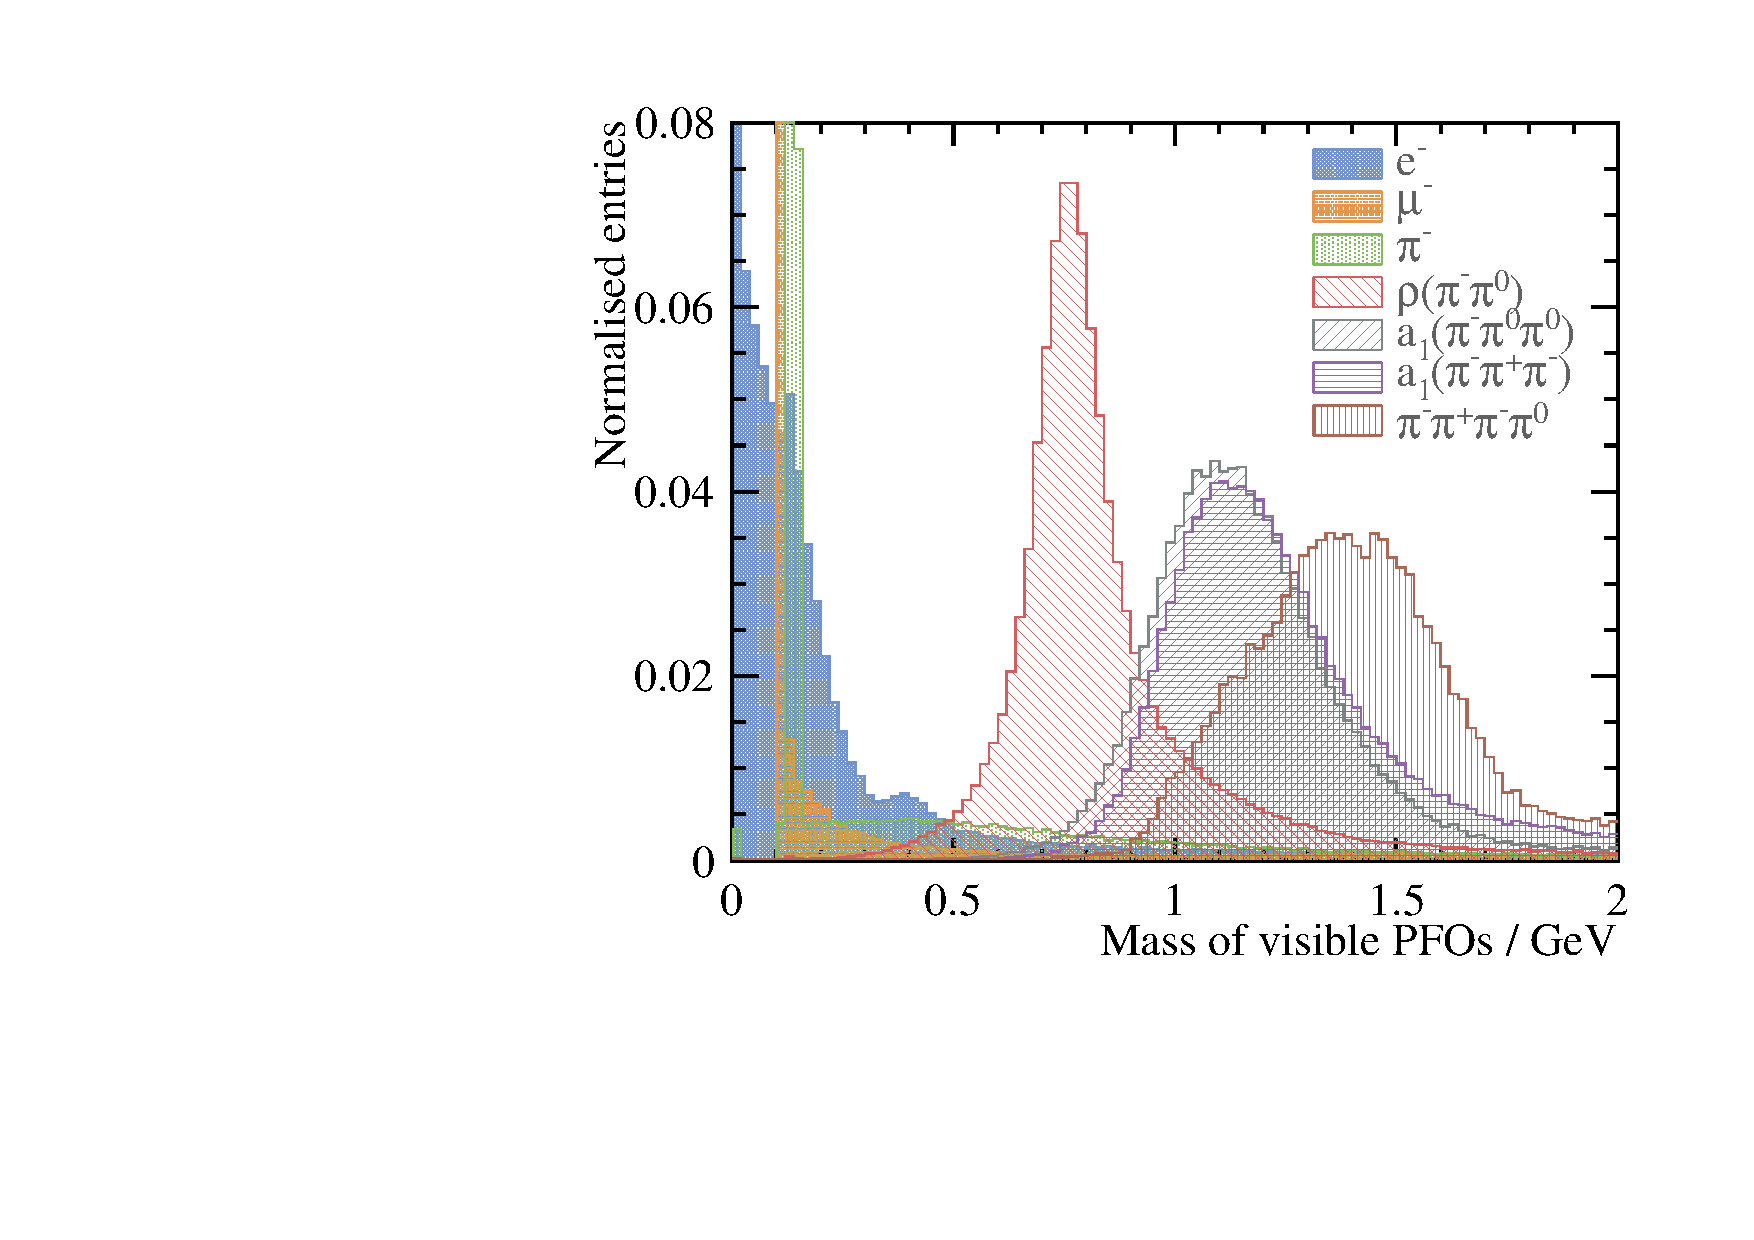
\includegraphics[width=\textwidth]{plots/var/mVis_100GeV_improved_zoom}
  \caption{}
  \label{fig:mVis}
\end{subfigure}
\hfill
\begin{subfigure}[b]{0.45\textwidth}
 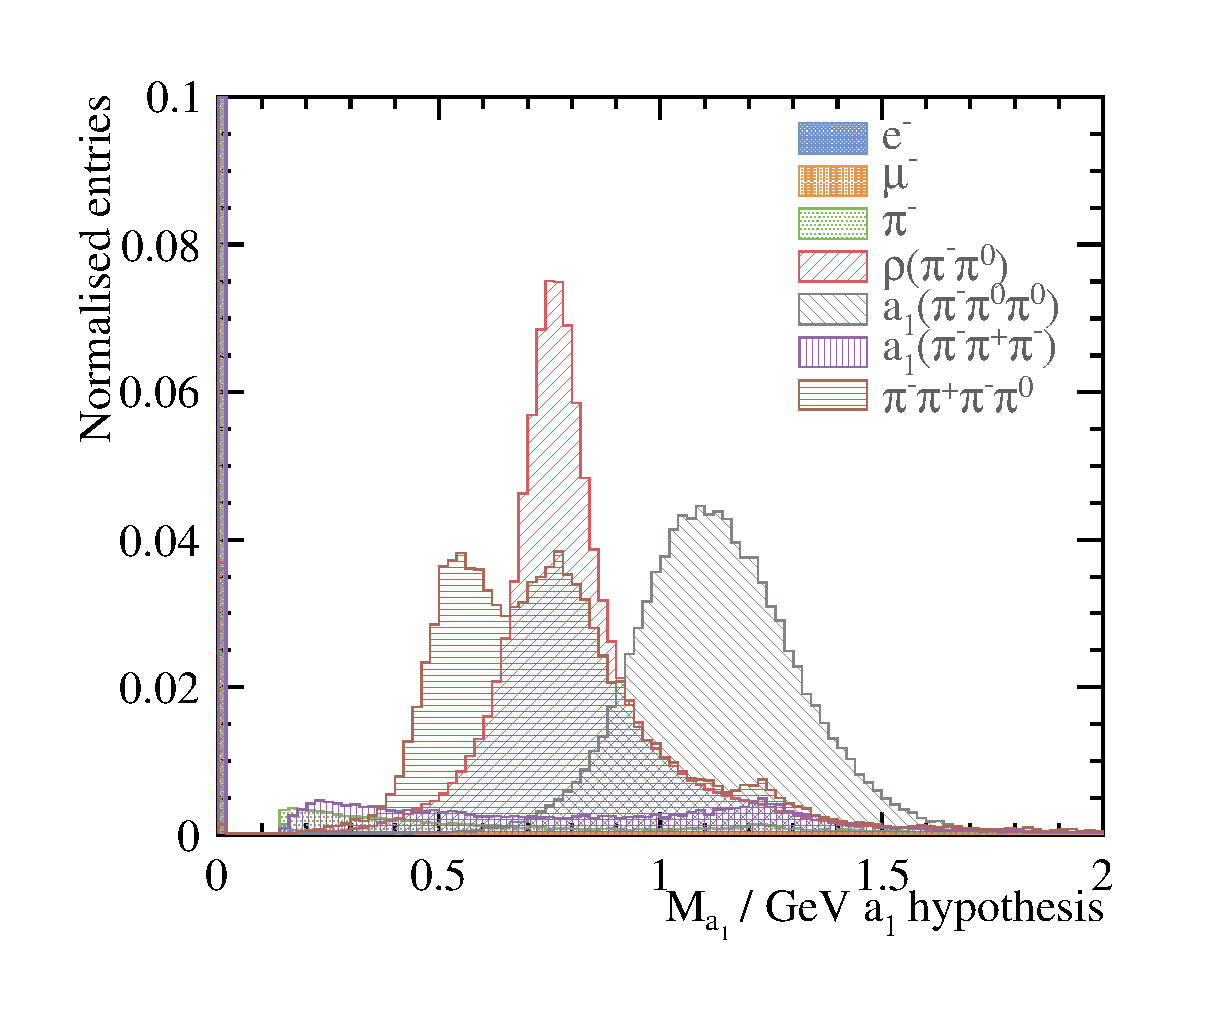
\includegraphics[width=\textwidth]{plots/var/mA1A1Fit_100GeV_improved_zoom}
  \caption{}
  \label{fig:mA1}
\end{subfigure}

\caption{Normalised distribution for discriminative variables for seven tau decay modes, \decayElectron, \decayMuon, \decayPion, \decayRho, \decayAiPhoton, \decayAiPion, and \decayThreePionPhoton,  with \rootS = 100 \,GeV for nominal CLIC\_ILD detector model. Figure~\ref{fig:nPfos} is the number of photons. Figure~\ref{fig:nCharge} is the number of charged PFOs. Figure~\ref{fig:mVis} is the invaraint mass of visible PFOs. Figure~\ref{fig:mA1} is the invaraint mass of \decayAiPhotonShort, calcuated with \decayAiPhotonShort hypothesis. 
}
\label{fig:var} 
\end{figure}

A set of discriminative variables were carefully developed, listed in the appendix. The reason for the large number of variables is due to training seven decay modes at once with the multvariate analysis, which will be discussed later. For the ease of dicussion and the similarity in event topologies, seven decay modes can be can be classified into three categories: leptonic decays, one-prong decays with photons and three-prong decays with photons. Leptonic decays refer to \decayElectron and \decayMuon. One-prong decays refer to \decayPion, \decayRho, and \decayAiPhoton. Three-prong decays refer to \decayAiPion and \decayThreePionPhoton.


%To identify the decay mode of \PGt from the decay products, a set of discriminative variables were carefully calculated and chosen. The full list of variables can be found in the appendix. There are 29 variables used in the multivariate analysis. The reason for the large number of variables is due to training seven decay modes at once, which will be discussed later.

%Some of the variables with most discriminative power are shown in figure~\ref{fig:nPfos}. 

The Number of photons is an important variable. It gives an excellent separation, due to excellent photon reconstruction provided by PandoraPFA. As shown in figure~\ref{fig:nPfos}, majority of \decayMuon, \decayPion and \decayAiPion final states have zero photon reconstructed. Nearly half of \decayElectron final state events have one photon reconstructed instead of zero, due to FSR. \decayRho and \decayThreePionPhoton have nearly 80\% events with two reconstructed photons, whilst \decayAiPion have over 60\% events with four reconstructed photons. The loss of photon reconstruction efficiency is because the difficulty of separating nearby photons.

The number of charged PFOs, shown in figure~\ref{fig:nCharge}, represent number of associate tracks to calorimeter cluters. It can clearly separate the leptonic and 1-prong final states, from the 3-prong final states. The charged PFO selection efficiency of leptonic final states are over 98\%.

The invariant mass of the visible PFOs, shown in figure~\ref{fig:mVis} is another powerful variable. \decayRho, \decayAiPhoton and \decayAiPion distributions show clear resonance at \PGrP{770} and \PaDoP{1260}. \decayElectron, \decayMuon and \decayPion distributions show much smaller invariant mass. \decayThreePionPhoton final state has a larger invariant mass than \PaDoP{1260}. The \decayElectron final state has a long tail of invariant mass due to extra photons from the FSR.

The resonance at \PGrP{770} and \PaDoP{1260}, shown in figure~\ref{fig:mVis}, can be further exploited to enhance the decay modes classification. For example, \decayAiPhoton decay mode has one \PGpm and four \PGg in the final state. By demanding two \PGg pairs having invariant mass close to that of a \PGpz, and  invariant mass of one \PGpm plus four \PGg close to that of a \PaDoP{1260}, resonace at \PaDoP{1260} is enhanced and the loss of efficiency in the reconstruction is compensated. In this example, if fewer than four \PGg are reconsrtructed, photon pairs would assume to merged in the reconstruction. This process would demand only one \PGg pair  having invariant mass close to that of a \PGpz, and invariant mass of one \PGpm plus all \PGg close to that of a \PaDoP{1260}. Simiarly, if there is fewer than  two \PGg, this process would just demand one \PGpm plus one \PGg having invariant mass close to that of a \PaDoP{1260}.

Formally, this resonance enhancement procedure is done via a $\chi^{2}$ minimisation. Using \decayAiPhoton final state as the exmaple, $\chi^{2}$ to minimise i defined as

\begin{equation}
\label{eq:a1}
\chi_{\Pa}^{2} = {\left(\frac{m_{\Pa,fit} -  m_{\Pa}}{\sigma_{\Pa}}\right)}^{2} + {\left(\frac{{m_{\PGpz,fit}} -  m_{\PGpz}}{\sigma_{\PGpz}}\right)}^{2} + {\left(\frac{{m_{\PGpz^*,fit}} -  m_{\PGpz}}{\sigma_{\PGpz}}\right)}^{2}  \,,
\end{equation}

where $m_{\PGpz,fit}$ and $m_{\PGpz^*,fit}$  are the invariant masses of all possible two photons combinations, $\sigma_{\Pa}$ and $\sigma_{\PGpz}$ are the half width of the invariant mass distribution of reconstructed \Pa and \PGpz using the truth information, and $m_{\Pa}$ and $m_{\PGp}$ are the masses of \Pa and \PGpz, taken from \cite{Agashe:2014kda}. This minisation, resonance enhancement sheme, for  \decayAiPhoton final state is called \decayAiPhoton hypothesis test, for short.

Figure~\ref{fig:mA1} shows the $m_{\Pa,fit}$ for \decayAiPhoton hypothesis test. \decayRho, \decayAiPhoton  and \decayThreePionPhoton final states contribute to the \Pa resonance, although only \decayAiPhoton final has a real \Pa resonance. 

For the \decayRho final state, a similar resonance enhancement scheme is used.


Additional variables include number of particles, energies, invariant mass of \PGmpm, \Pepm, \PGg and charged PFOs. Futher separation between \decayElectron and \decayPion decay states are improved with calorimeter information. The information includes comparison of observed and expected electromagnetic shower profile, the maching between inner detector tracks and calorimeter clusters, and the fraction of calorimeter hits registered as minimum ionised particles.


%Additional variables are calculated using the calorimeter information, the comparison with the electromagnetic shower profile, the matching between the track and the cluster, the energy and invariant masses for different types of particles. Extra variables regarding to the electromagnetic shower profile are used to distinguish electrons from charged pions.

%, listed in Table XX. Note that XX variables were specialised in separating a electron from a pion. XX variables were made to test the hypothesis of XX particles. The rho hypothesis is to find the best rho decay candidates by minimising chi squared according to $aa$, where X is all possible charge pions, Y is all possible 2 photons. The formula will reduce accordingly if there is 1 photon. Similarly, the a1 decaying to 1 pion 4 photon hypothesis is done in a same fashion with Chi squared function XX, , where X is all possible charge pions, Y is all possible 2 photons. The formula will reduce accordingly if there are 2 or 3 photons.

%The variables of energy ratios instead of the raw energies were calculated to make the MVA process more generic across different c.o.m. energies.

For the multivariate analysis, the multiclass of the TMVA package \cite{Therhaag:2009dp} was used to perform a multiclass classification, which trains the seven final states simultaneously. The multiclass class is an extension of the standard two-class signal-background classifier. For each final state, the multiclass classifier will train the final state as the signal against all other final states as the background. This process is repeated for each final state. The classifier output for a single event is a normalised response for each final state, where the sum is one. The response of each final state of a event can be treated as the likelihood. The event is classified into a particular final state if the final state has the highest classifier output response. The advantage of using the multiclass is that the correlation between different final states are accounted for and the classifier output are correctly adjusted for multiple final states, hence one event can only be classified into one final state. The issue with the multiclass is that discriminative variables for each final state need enter the training stage, resulting in a large number of variables. 

Half of the events, randomly selected, were used in the training process and the other half were used for testing. The TMVA multiclass classifier is a boosted decision tree with gradient boosting (BDTG), as it was found to give for the best performance. The MVA classifier is trained and optimised to give the best overall separation across all final states.

\section{Results}

\begin{table}[htbp]
\centering
\caption{\label{tab:sel_example} Classification probability for tau decay modes in columns in percentage of \rootS = 100 \,GeV in the nominal CLIC\_ILD detector model. Bold numbers show the correctly reconstructed terms. Numbers less than 0.25\% are not shown. Statistical uncertainties are less than 0.25\%. \PGnGt in final states are not shown.}
\smallskip
\small
\begin{tabular}{| l | r | r | r | r | r | r | r |}
\hline
  \textbf{Reco $\downarrow$ True $\to$}  & \textbf{\decayElectronShort} & \textbf{\decayMuonShort} &\textbf{\decayPionShort} & \textbf{\decayRhoShort} &\textbf{\decayAiPhotonShort} &\textbf{\decayAiPionShort} &\textbf{\decayThreePionPhotonShort} \\
\hline

\textbf{\decayElectronShort}&\textbf{99.8}&-&0.9&1.1&0.8&-&-\\
\textbf{\decayMuonShort}&-&\textbf{99.5}&0.5&-&-&-&-\\
\textbf{\decayPionShort}&-&0.3&\textbf{93.2}&0.9&-&0.4&-\\
\textbf{\decayRhoShort}&-&-&4.1&\textbf{93.0}&10.5&0.6&2.8\\
\textbf{\decayAiPhotonShort}&-&-&-&4.3&\textbf{88.2}&-&1.0\\
\textbf{\decayAiPionShort}&-&-&1.0&0.3&-&\textbf{96.6}&6.9\\
\textbf{\decayThreePionPhotonShort}&-&-&-&0.4&0.4&2.4&\textbf{89.3}\\

\hline
\end{tabular}
\end{table}

Table~\ref{tab:sel_example} shows classification probabilities for seven tau decay final states of 100 \,GeV in  the nominal CLIC\_ILD detector model. An ideal reconstruction would have diagonal terms in the table. 

%The reconstruction efficiencies for the seven final state of the tau decaying with c.o.m. energy of 100 \,GeV for the nominal CLIC\_ILD detector are shown in the 
%For the leptonic decays, the correct classifiction probabilities are above 99.5\%, aided by the tracking system, which offers precision position and momentum measurements.

The \decayMuonShort final state has very clear topology, as muon deposits energy in the muon chamber. Therefore, there is little confusion with other final states.

\decayElectronShort final state is well separated, due to variables aimed to differentiate early hadronic shower to electromagnetic shower. 

For the leptonic decays, the correct classifiction probabilities are above 99.5\%, aided by the tracking system, which offers precision position and momentum measurements

For one prong final states, \decayPionShort, \decayRhoShort, and \decayAiPhotonShort, the confusion is mainly due to the inability to separate two neabrby photons originated form \Ppizero, which is limited by the calorimeter spatial resolution.. 

Similarly the confusion between 3-prong final state, \decayAiPionShort, and \decayThreePionPhotonShort is caused by same inability to resolove two nearby photons.

Overall a rather high correct classification probability for each tau decay mode is achieved. 

\section{Electromagnetic caloritmeter optimisation}

The classification was with  \rootS = 100, 200, 500, 1000 GeV. The ECal square cell sizes were varied at 3, 5, 7, 10, 15 and 20\,mm, whilst keeping other ECal dimention constant. 

\begin{figure}[htbp]
\centering % \begin{center}/\end{center} takes some additional vertical space

\begin{subfigure}[b]{0.45\textwidth}
  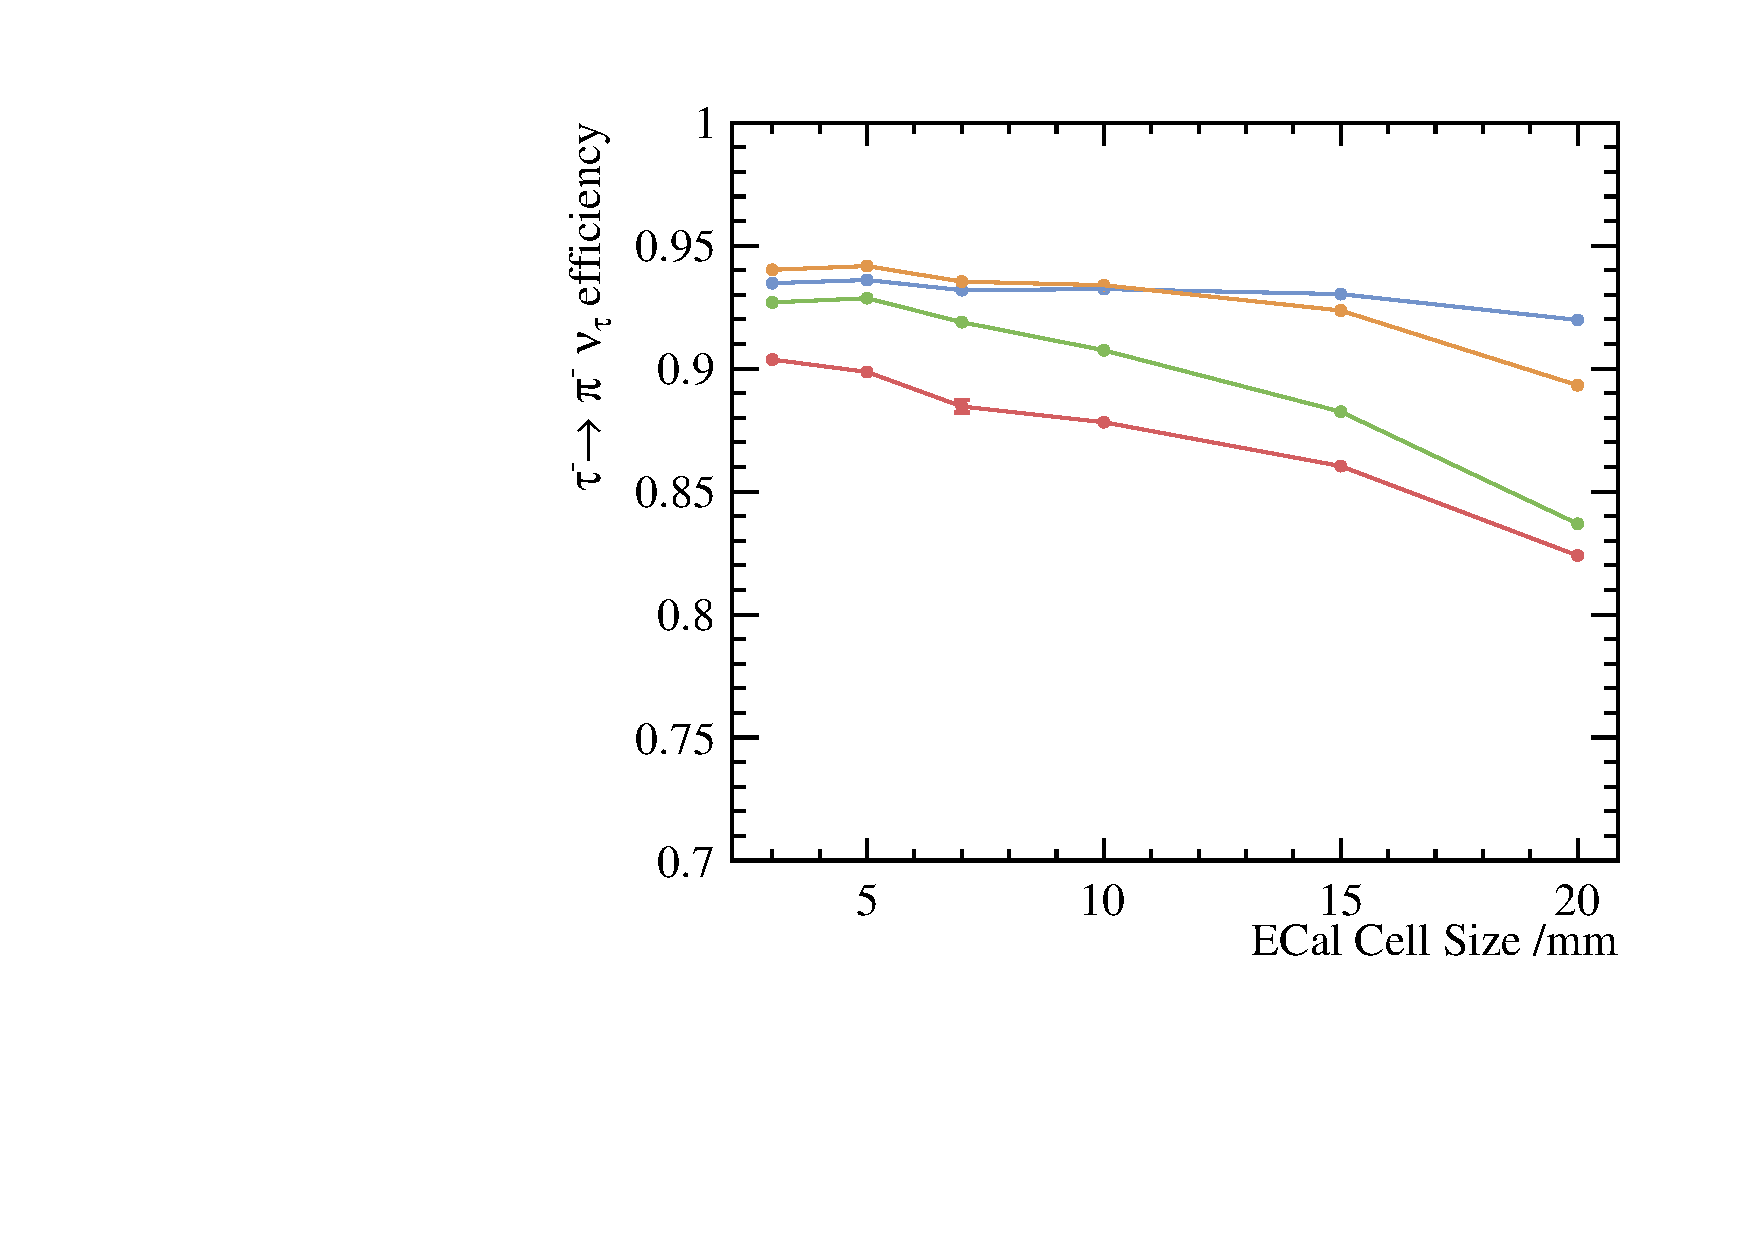
\includegraphics[width=\textwidth]{plots/decayMode2}
  \caption{}
  \label{fig:decayMode2}
\end{subfigure}
\hfill
\begin{subfigure}[b]{0.45\textwidth}
  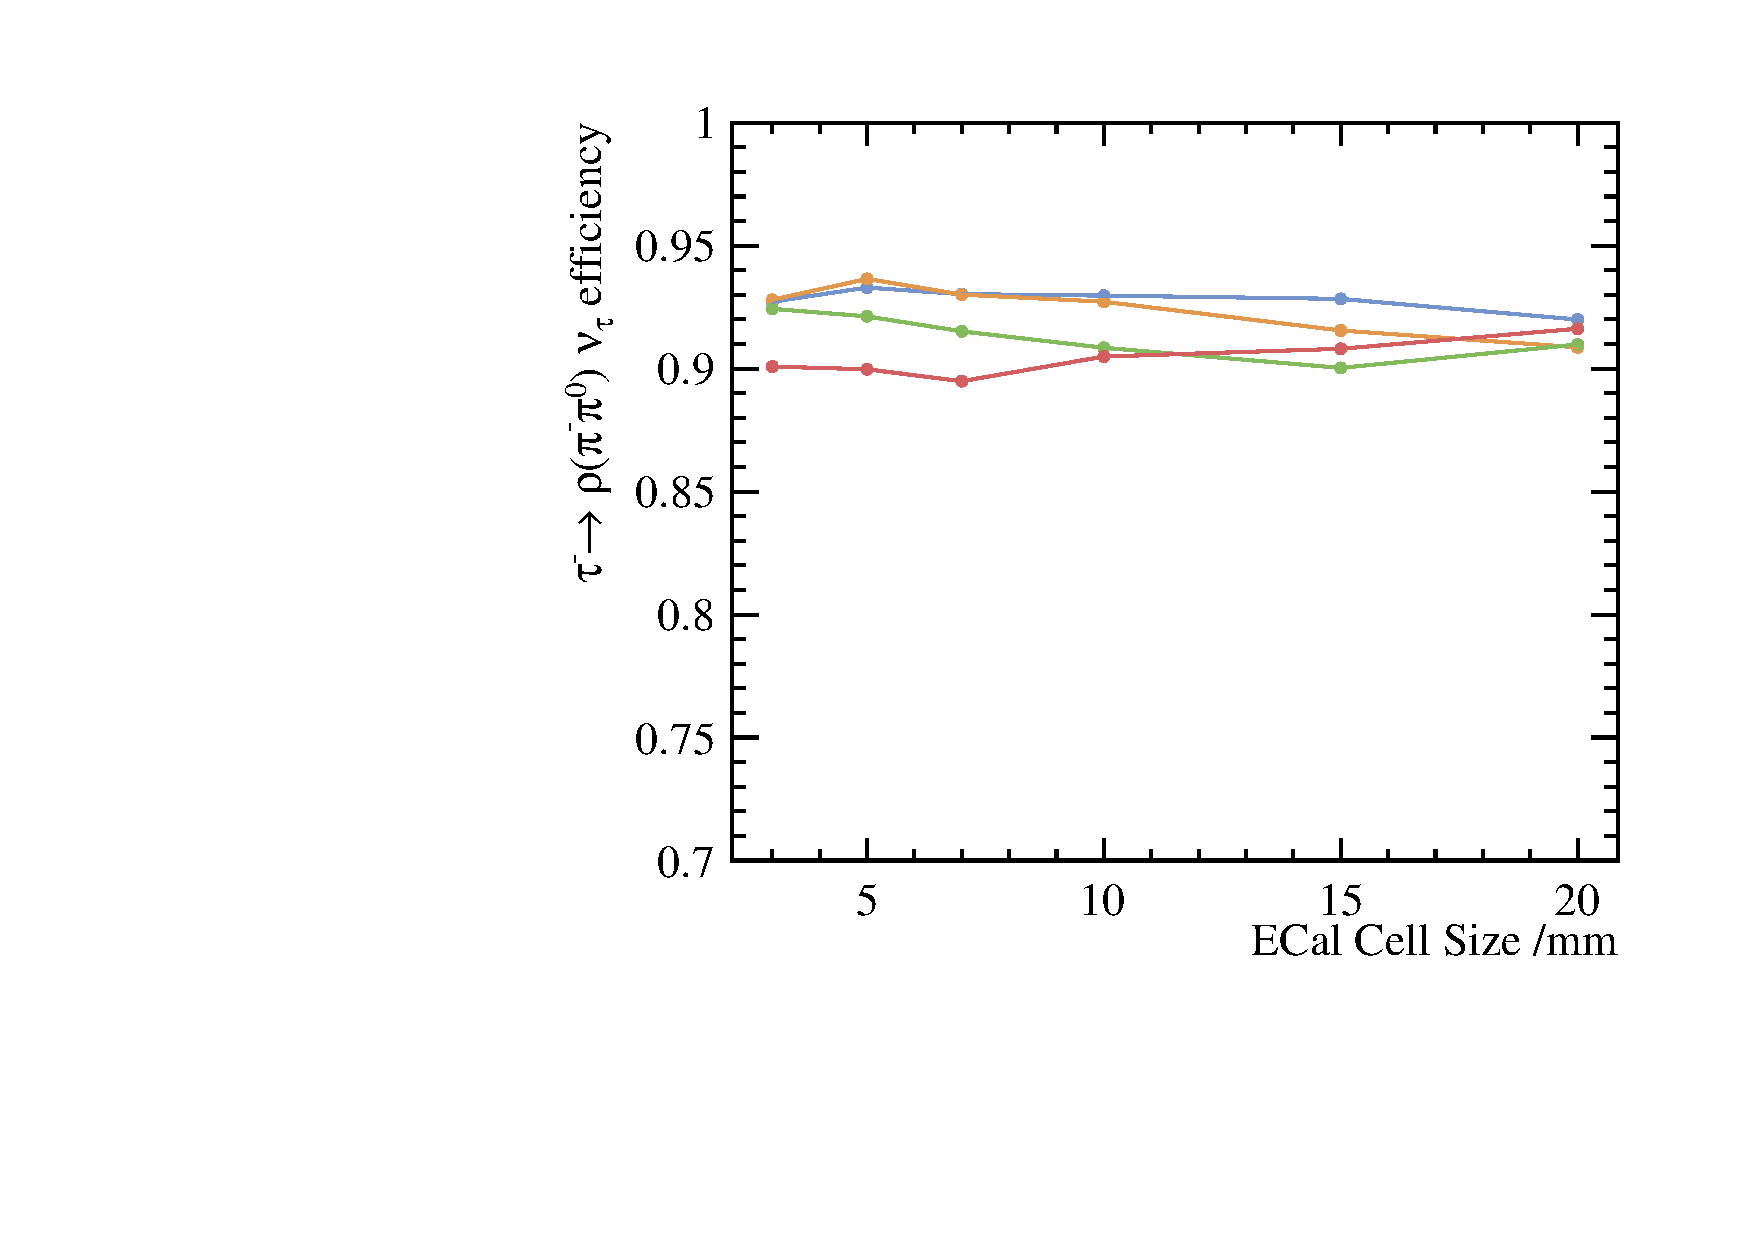
\includegraphics[width=\textwidth]{plots/decayMode3}
  \caption{}
  \label{fig:decayMode3}
\end{subfigure}


\begin{subfigure}[b]{0.45\textwidth}
  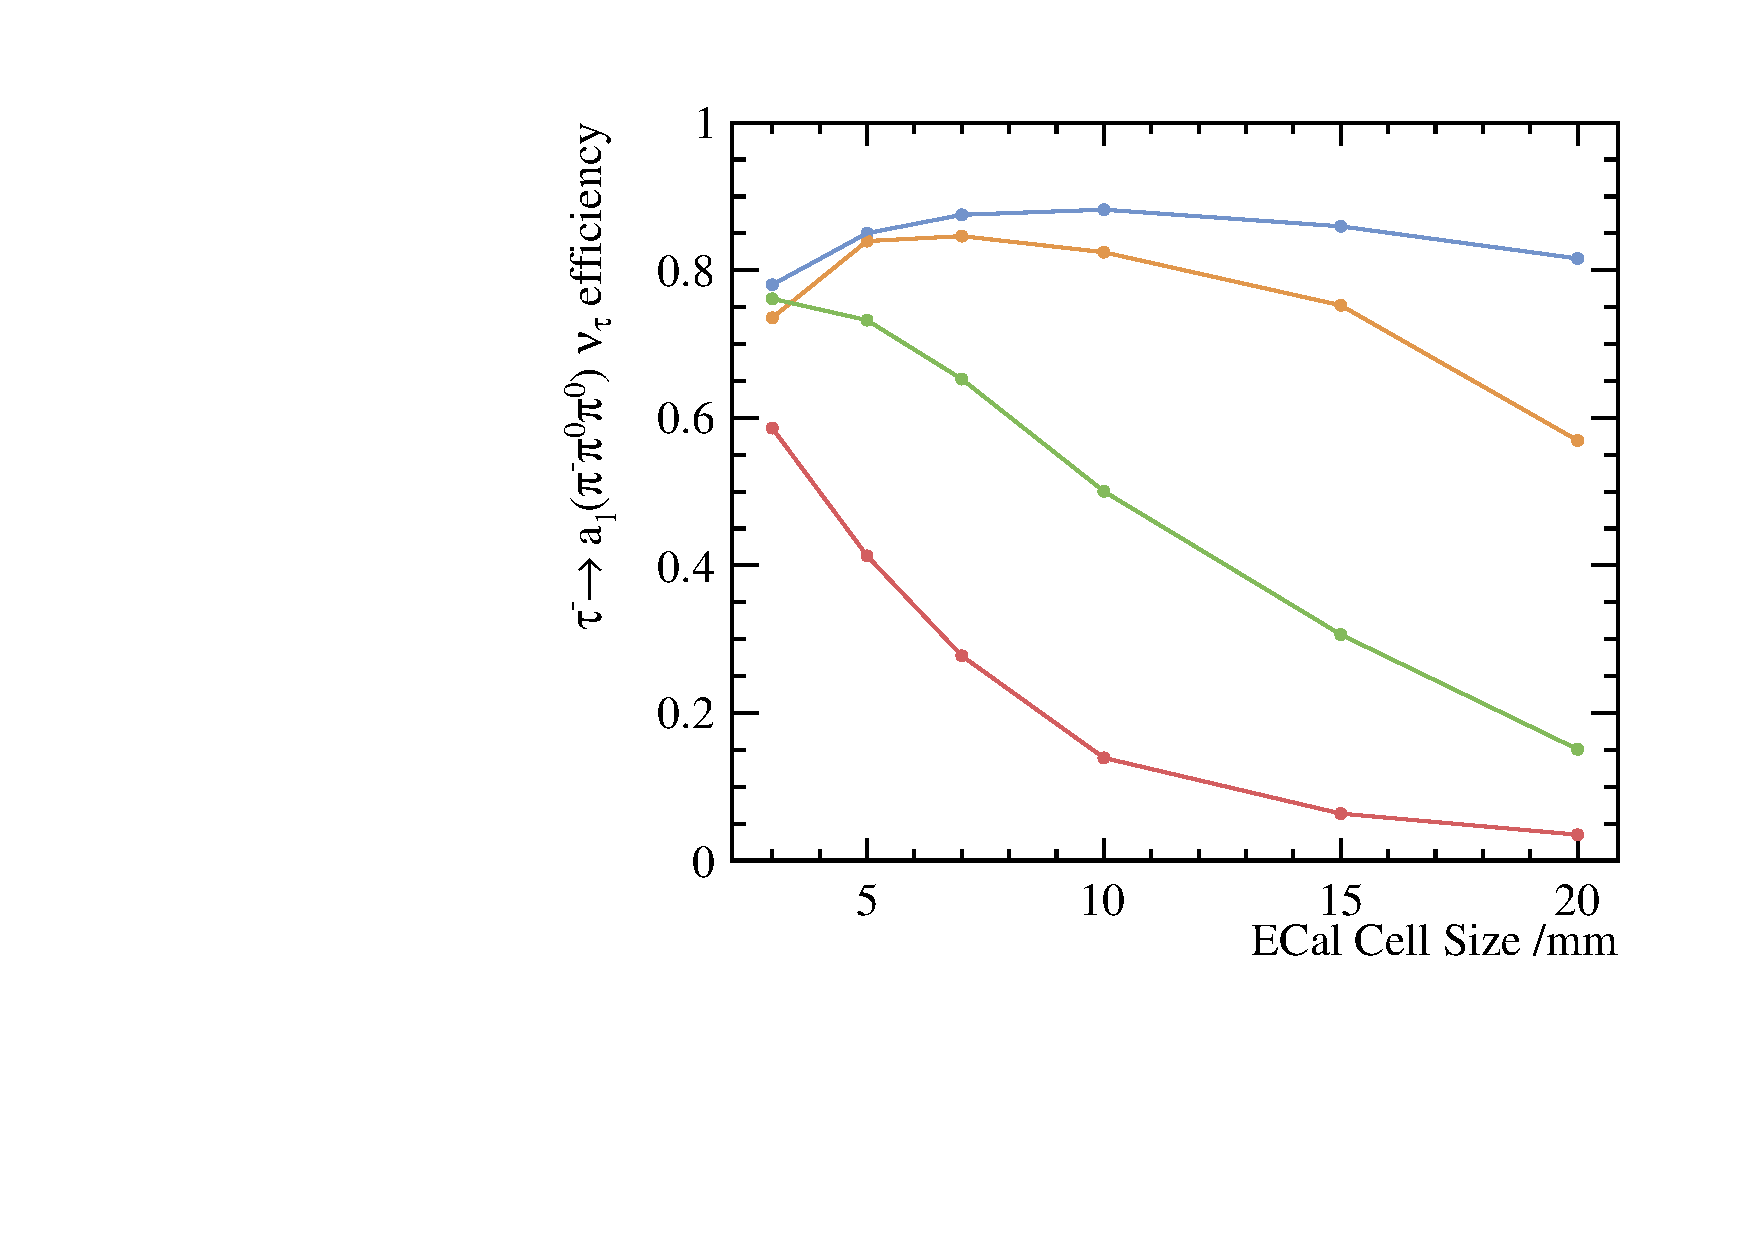
\includegraphics[width=\textwidth]{plots/decayMode4}
  \caption{}
  \label{fig:decayMode4}
\end{subfigure}
\hfill
\begin{subfigure}[b]{0.45\textwidth}
  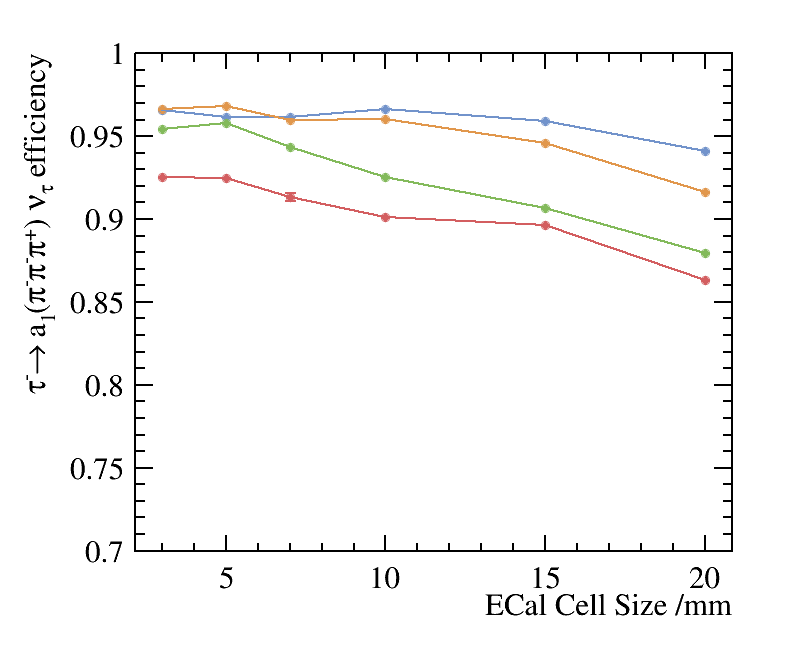
\includegraphics[width=\textwidth]{plots/decayMode5}
  \caption{}
  \label{fig:decayMode5}
\end{subfigure}


\begin{subfigure}[b]{0.45\textwidth}
  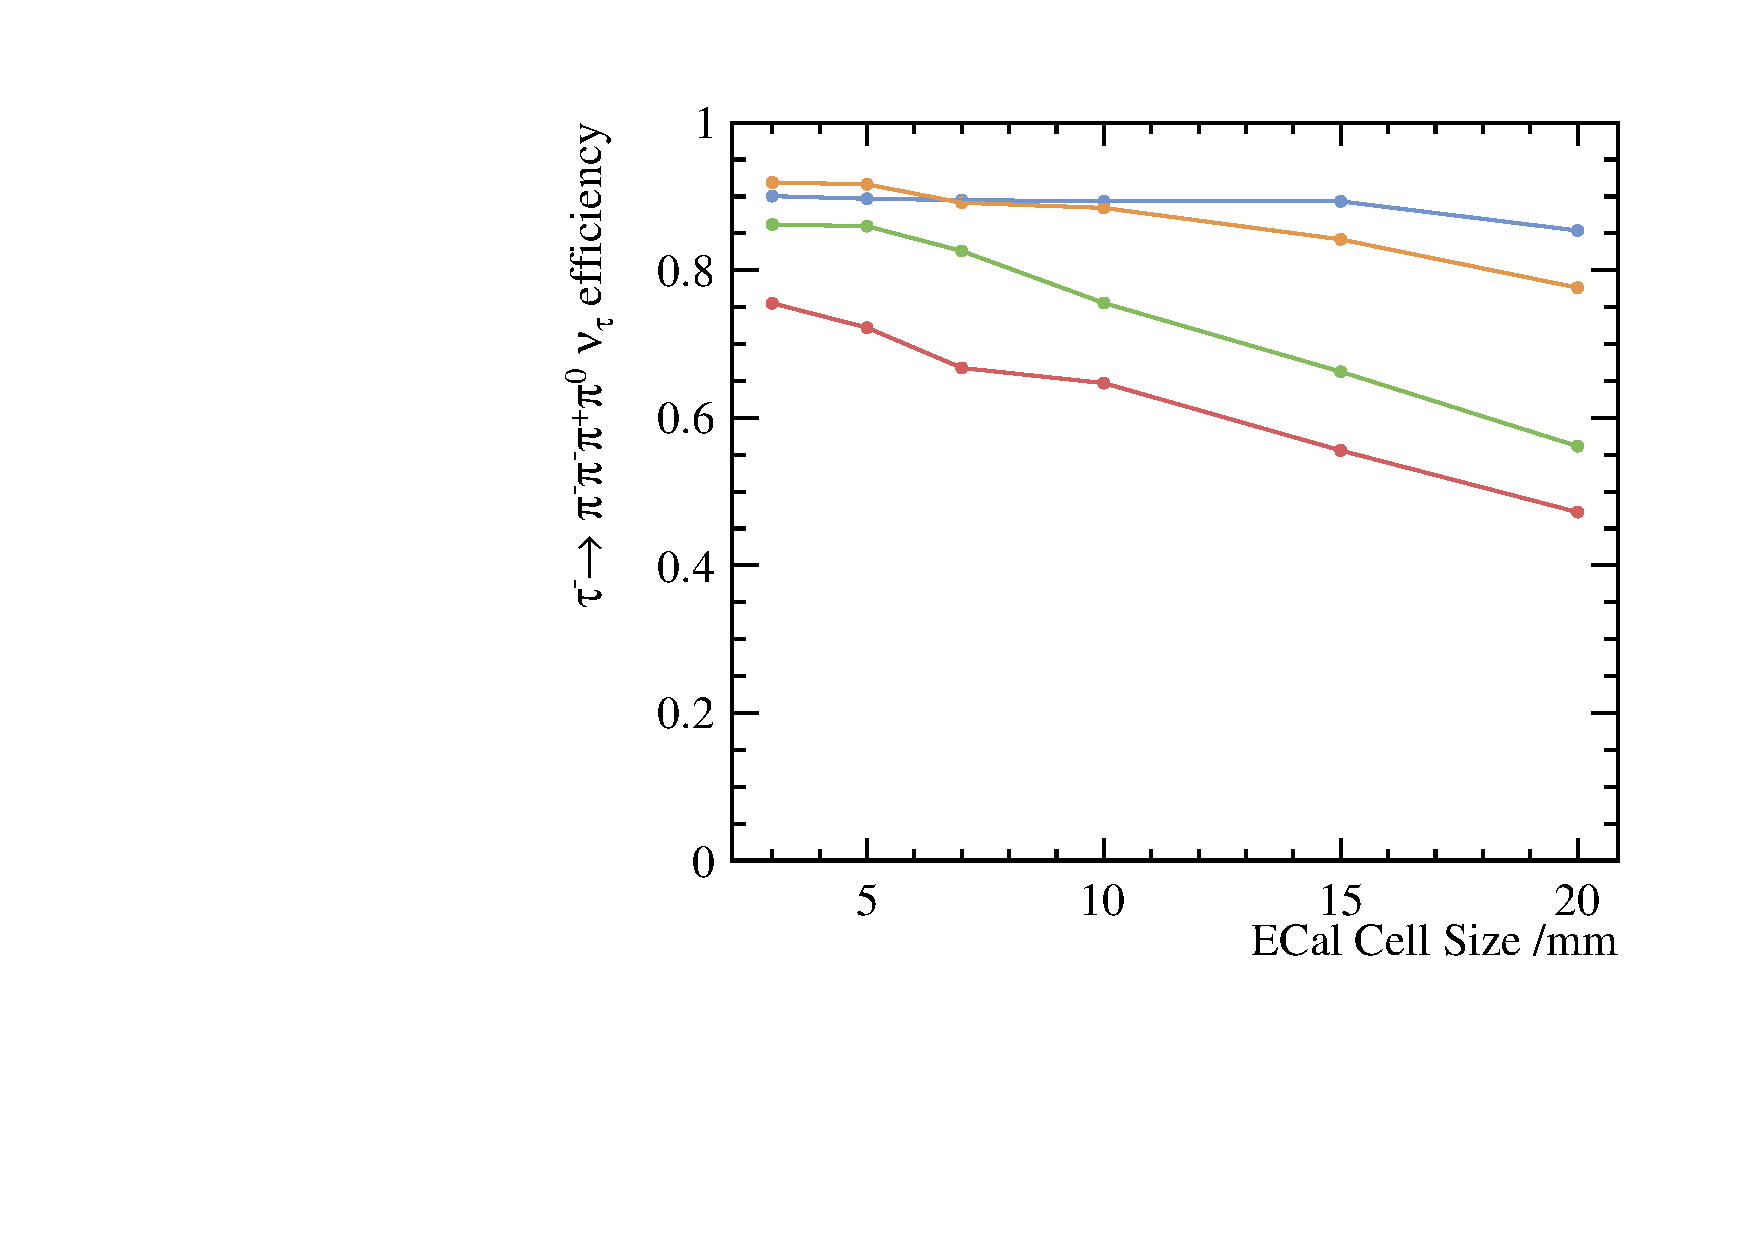
\includegraphics[width=\textwidth]{plots/decayMode6}
  \caption{}
  \label{fig:decayMode6}
\end{subfigure}
\hfill
\begin{subfigure}[b]{0.45\textwidth}
  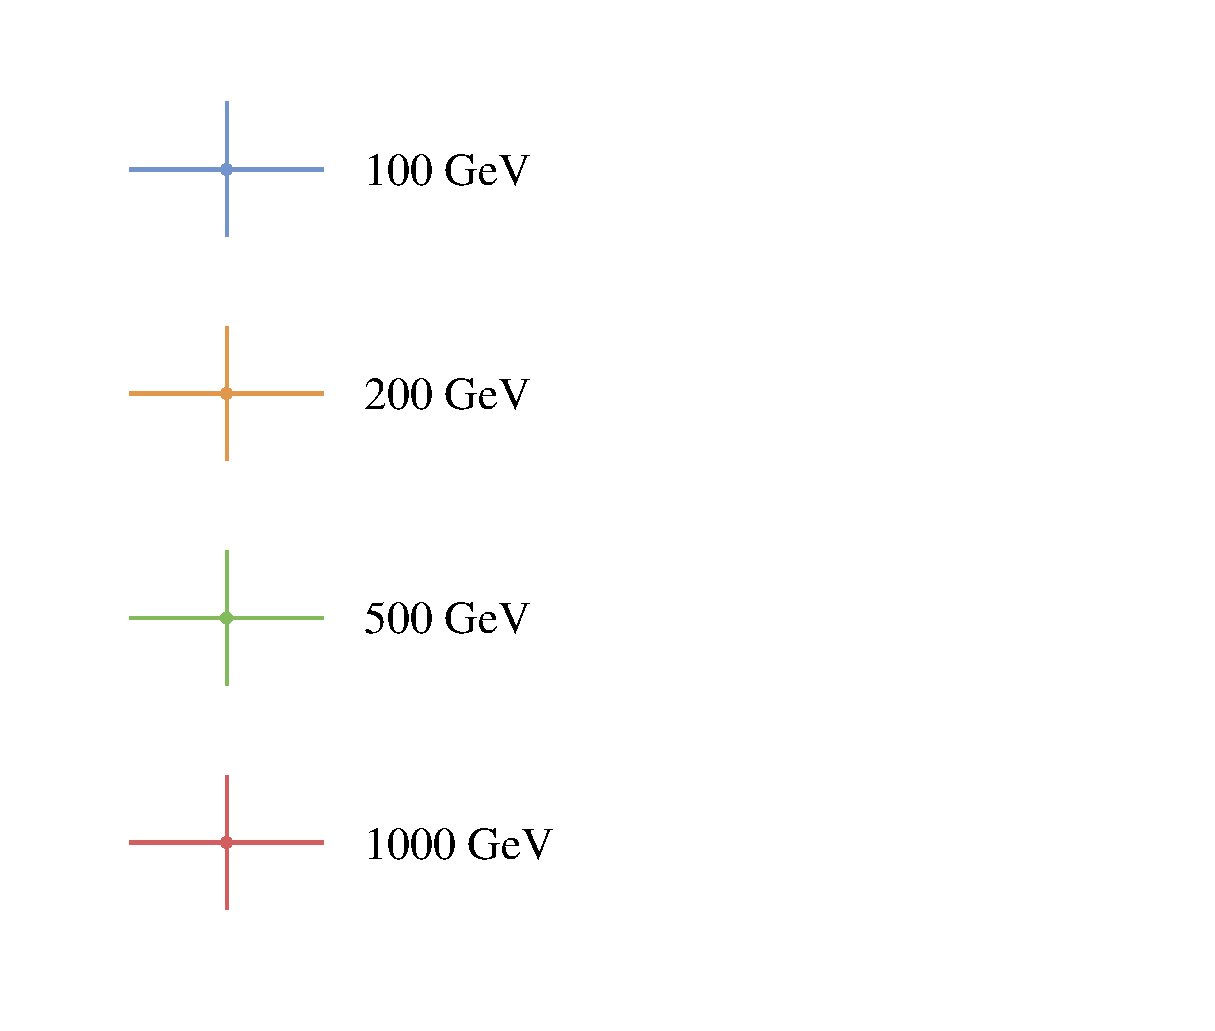
\includegraphics[width=\textwidth]{plots/legend}
  %\caption{}
  %\label{fig:legend}
\end{subfigure}

%\qquad
%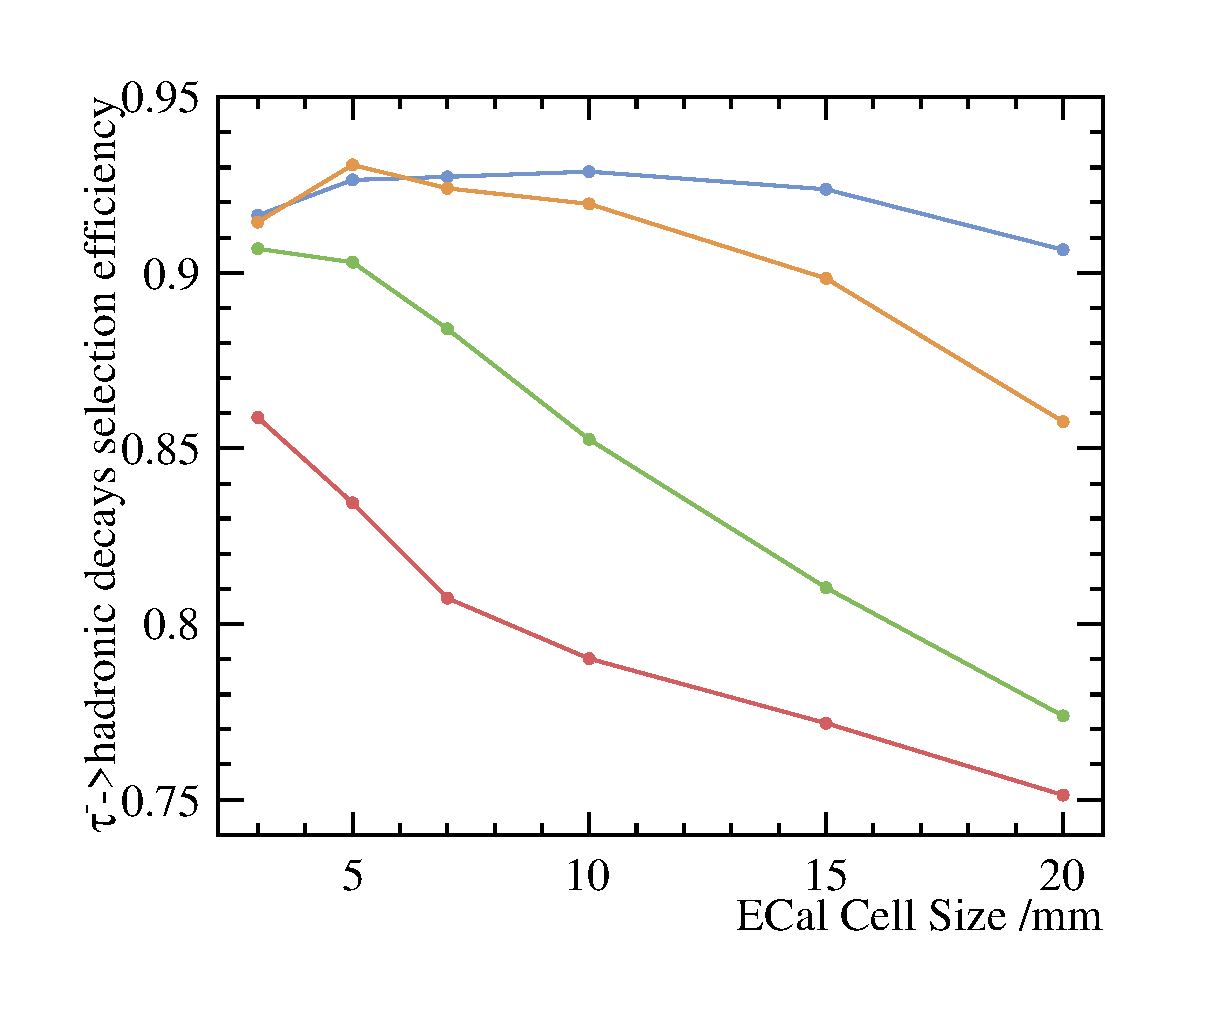
\includegraphics[width=.4\textwidth]{plots/hadEff}
% "\includegraphics" from the "graphicx" permits to crop (trim+clip)
% and rotate (angle) and image (and much more)
\caption{\label{fig:pion_efficiency} The correct classcification probabilities for various final states against the ECal cell size of different c.o.m. energies in the nominal CLIC\_ILD detector model. Figure~\ref{fig:decayMode2}, ~\ref{fig:decayMode3}, ~\ref{fig:decayMode3}, ~\ref{fig:decayMode4}, ~\ref{fig:decayMode5} are for the \decayPion, \decayRho,  \decayAiPhoton, \decayAiPion  and \decayThreePionPhoton  final states, respectively. Blue, orange, green and red lines are representing  \rootS = 100, 200, 500 and 1000\,GeV respectively. Note that the y axis are not all the same, for display purposesy.}
\end{figure}

The impact of the ECAL cell sizes and the \rootS energies on the classification probabilities of tau decay modes are shown in figure~\ref{fig:pion_efficiency}. The correct classification probabilities of leptonic decays are not shown, as they are similar across different ECal cell sizes. This is because the \Pepm and \PGmpm identifications mostly rely on the inner detector tracking system, which does not vary in this study. The energy deposited in the calorimeter are used for the association to the inner detector tracks, but it has a small impact on the lepton identification. 

Overall, the correct classification probabilites of hadronic decays decrease as the \rootS energy increases. Taus are boosted at higher \rootS, the separation between decay products is smaller. Hence it is more difficult to reconstruct multi-particle final states correctly.

The correct classification probabilites decrease as the ECal square cell size increases. Larger cell sizes means that the ECal offers a lower spatial resolutions, making the separation of nearby particles more difficult.



For the \decayRho final state, the correct classification probabilites for \rootS = 500\,GeV rises for ECal sqaure cell sizes from 15 to 20\,mm, and for  \rootS = 1000\,GeV from 7, to 20\,mm. This is compensated with the sharp drop in correct classification probabilites for the \decayAiPhoton final state in the same \rootS and the same energy. When reconstruction fails to separate nearby photons, the event topologies of two final states are very similar.



For \rootS = 100 and 200\,GeV, the correct classification probabilites for the 5\,mm ECal cell size is better than that of the 3\,mm. One possible explanation is that the PandoraPFA have been optimised for the nominal ILD detector with the 5\,mm ECal cell size, which shares the same ECal structure with the nominal CLIC\_ILD detector.



\begin{figure}[htbp]
\centering % \begin{center}/\end{center} takes some additional vertical space
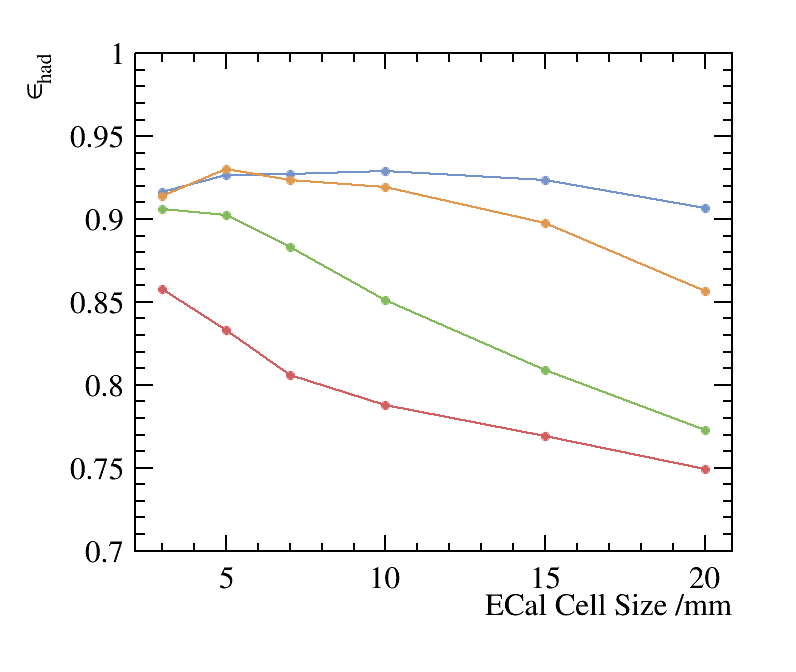
\includegraphics[width=.45\textwidth]{plots/hadEff3}
% "\includegraphics" from the "graphicx" permits to crop (trim+clip)
% and rotate (angle) and image (and much more)
\caption{\label{fig:hadronic_efficiency} The tau lepton hadronic decay correct classification probability as a function of the ECal sqaure cell size for different \rootS,   in the nominal CLIC\_ILD detector model. Blue, orange, green and red lines represent \rootS = 100, 200, 500 and 1000\,GeV, respectively.}
\end{figure}

Overall classification performance across all decay modes can be compared by constructing a single parameter function, which is a weighted average of correct classification probability for each decay modes. This single parameter allows the direct comparison between different ECal cell sizes, for different \rootS. It represents an overall classification performance, which MVA is optimised to.

Formally, the chosen single parameter function is the tau lepton hadronic decay correct classification probability, $\varepsilon_{had}$, which is defined as
\begin{equation}
\label{eq:had}
\varepsilon_{had} = \frac{\left(\Sigma_{i} {Br}_{i}\varepsilon_{i}\right)}{\Sigma_{i} {Br}_{i}}  \,,
\end{equation}
where $Br_{i}$ is the branching ratio of a hadronic decay mode after the generator level cut in section~\ref{section:MC}. $\varepsilon_{i}$ is the correct classcification probability for decay mode $i$. Summation is over five hadronic decay modes. Leptonic decays, \decayElectron and \decayMuon, were not included because the variations in the leptonic decay correct classcification probabilities are small.


Figure~\ref{fig:hadronic_efficiency} shows the tau lepton hadronic decay correct classification probability, $\varepsilon_{had}$, as a function of the ECal sqaure cell size for different \rootS in the nominal CLIC\_ILD detector model. $\varepsilon_{had}$ decreases when ECal square cell sizes increases, and when \rootS increases.

For \rootS = 100 and 200\,GeV, $\varepsilon_{had}$ for the 5\,mm ECal square cell size is better than that of the 3\,mm. This is possibly due the optimisation of the software for the nominal ILD 5\,mm square cell size.

ECal square cell size has a bigger impact on higher \rootS. For \rootS = 100\,GeV, $\varepsilon_{had}$ is above 90\%. For \rootS = 200\,GeV, $\varepsilon_{had}$ decreases from over 90\% to 86\% for ECal square cell sizes from 3 to 20\,mm. For \rootS = 500 and 1000\,GeV, $\varepsilon_{had}$ degrades significantly, from over 90\% to 77\%,  and from 86\% to 75\%, respectively, for the same range of the cell sizes. 

%For low \rootS, namely 100 and 200\,GeV, up to 15\,mm cell sizes of ECal will give a good performance for \PGt hadronic decay modes separation, and the $\varepsilon_{had}$ is above 90\%. For the high c\rootS, namely 500 and 1000\,GeV, it is preferential to have a small ECal cell size for \PGt hadronic decay modes separation. There is about 15\% degradation of $\varepsilon_{had}$ for ECal cell size from 3 to 20\,mm.

%The degradation of $\varepsilon_{hadronic}$ is more significant for higher c.o.m. energy.

%The paper illustrated the usage of reconstruction of the tau decay modes as a benchmark for the detector optimisation. 

%The high probability of correctly identifying the decay modes also showed the potential to measure the spin of the {\Ptau} with the CLIC machine.


%We discourage the use of inline figures (wrapfigure), as they may be
%difficult to position if the page layout changes.

%We suggest not to abbreviate: ``section'', ``appendix'', ``figure''
%and ``table'', but ``eq.'' and ``ref.'' are welcome. Also, please do
%not use \texttt{\textbackslash emph} or \texttt{\textbackslash it} for
%latin abbreviaitons: i.e., et al., e.g., vs., etc.



%\section{Sections}
%\subsection{And subsequent}
%\subsubsection{Sub-sections}
%\paragraph{Up to paragraphs.} We find that having more levels usually
%reduces the clarity of the article. Also, we strongly discourage the
%use of non-numbered sections (e.g.~\texttt{\textbackslash
%  subsubsection*}).  Please also see the use of
%``\texttt{\textbackslash texorpdfstring\{\}\{\}}'' to avoid warnings
%from the hyperref package when you have math in the section titles



\appendix
\section{Variables for multivariate analysis}

Here is a full list of all variables used in the multivariate analysis. Energy of the \PGt is assume to be the same as the energy of \Pepm beam, which is half of the \rootS energy. Recoil momenta were calculated assuming the \Pem\Pep collision happened at the centre of mass energy. 
%Both assumptions are largely valid when there is no ISR contribution.

\begin{itemize}
\item  $\frac{E_{ECal,HCal}}{E_{tot}}$, charged:  Sum of energy deposited in ECal and HCal, divided by the energy of charged PFOs  
\item  $\frac{E_{ECal,HCal}}{E_{tot}}$, all:  	 Sum of energy deposited in ECal and HCal, divided by the energy of all PFOs  
\item  $m_{vis}$:     	 Invariant mass of visible particles in GeV   
\item  $\frac{E_{vis}}{E_{\PGtm}}$:	 Sum of energy of all PFOs, divided by the energy of \PGtm 
\item  $\frac{E_{charged}}{E_{\PGtm}}$:	 Sum of energy of charged PFOs, divided by the energy of \PGtm    
\item  $\frac{E_{\PGmm}}{E_{\PGtm}}$:	 Sum of energy of muons, divided by the energy of \PGtm    
\item  $\frac{E_{\Pem}}{E_{\PGtm}}$:	 Sum of energy of electrons, divided by the energy of \PGtm
\item  $\frac{E_{\PGg}}{E_{\PGtm}}$:	 Sum of energy of photons, divided by the energy of \PGtm  
\item  $\frac{E_{\PGpm}}{E_{\PGtm}}$:	 Sum of energy of charged pions, divided by the energy of \PGtm    
\item  $N_{charged}$:	 Number of charged PFOs    
\item  $N_{\PGmm}$:	 Number of muons    
\item  $N_{\Pem}$:	 Number of electrons
\item  $N_{\PGg}$:	 Number of photons  
\item  $N_{\PGpm}$:	 Number of charged pions    
\item  $m_{\PGg}$:     	 Invariant mass of photons in GeV   
\item  $m_{charged}$:     	 Invariant mass of charged PFOs in GeV   
\item  $m_{neutral}$:     	 Invariant mass of neutral PFOs in GeV   
\item  $m_{\PGpm}$:     	 Invariant mass of charged pions in GeV   
\item  $m_{\PGpz}, \PGrP{\PGpm\PGpz}$ hypothesis:     	 Fitted invariant mass of \PGpz for \PGrP{\PGpm\PGpz} hypothesis test  
\item  $m_{\PGrP{\PGpm\PGpz}}, \PGrP{\PGpm\PGpz}$ hypothesis:     	 Fitted invariant mass of \PGr for \PGrP{\PGpm\PGpz} hypothesis test  

\item  $m_{\PGpz, 1}, \PaDoP{\PGpm\PGpz\PGpz}$ hypothesis:     	 First fitted invariant mass of \PGpz, for \PaDoP{\PGpm\PGpz\PGpz} hypothesis test, ordered by closeness to the true \PGpz mass  
\item  $m_{\PGpz, 2}, \PaDoP{\PGpm\PGpz\PGpz}$ hypothesis:     	 Second fitted invariant mass of \PGpz, for \PaDoP{\PGpm\PGpz\PGpz} hypothesis test, ordered by closeness to the true \PGpz mass  
\item  $m_{\PaDoP{\PGpm\PGpz\PGpz}}, \PaDoP{\PGpm\PGpz\PGpz}$ hypothesis:     	 Fitted invariant mass of \PaDoP{\PGpm\PGpz\PGpz}, for \PaDoP{\PGpm\PGpz\PGpz} hypothesis test 
\item  $\overline{E_{cell}}$:     	 Average energy deposited in a calorimeter cell in GeV 
\item  $d_{trans,shower}$:    Transverse shower width for electromagnetic shower profile, averaged for all clusters in the ECal 
\item  $l_{long,shower}$:    Longitudinal start layer for electromagnetic shower profile, averaged for all clusters in the ECal 
\item  $\Delta{l_{long,shower}}$:    Longitudinal discrepancy for electromagnetic shower profile, averaged for all clusters in the ECal 
\item  $\%MIP$:    Fraction of calorimeter hits registered as minimum ionised particles, averaged for all clusters in the ECal 
\item  $\frac{E}{P}$:   Energy divided by momentum, averaged for all clusters in the ECal 
\end{itemize}

\acknowledgments

The authors would like to thank P. G. Roloff for helping to generate the simulated samples. 

%\paragraph{Note added.} This is also a good position for notes added
%after the paper has been written.





% We suggest to always provide author, title and journal data:
% in short all the informations that clearly identify a document.

\bibliographystyle{h-physrev3}
\bibliography{bib}

%\begin{thebibliography}{99}

%\bibitem{a}
%Author, \emph{Title}, \emph{J. Abbrev.} {\bf vol} (year) pg.

%\bibitem{b}
%Author, \emph{Title},
%arxiv:1234.5678.

%\bibitem{c}
%Author, \emph{Title},
%Publisher (year).


% Please avoid comments such as "For a review'', "For some examples",
% "and references therein" or move them in the text. In general,
% please leave only references in the bibliography and move all
% accessory text in footnotes.

% Also, please have only one work for each \bibitem.


%\end{thebibliography}


\end{document}
